\subsection{Dependencies}
In this part of the document we will discuss the relationships between the architectural components of the system and how they are dependent on one another. A software entity \verb!A! is dependent on a software entity \verb!B! when it makes use of \verb!B! either by referencing it directly, calling \verb!B!'s methods, instantiating \verb!B! or returning instances of \verb!B! in its own methods. We have noted two types of dependencies throughout the system: intra-component dependencies and inter-component dependencies. The formes ones exist among the sub-component of every architectural components of OptaPlanner individually, whereas the latter ones exist between the components themselves. 
\subsubsection{Intra-component dependencies}
The three architectural components of OptaPlanner - API, the Implementation System and the Configuration system - have a substantial amount of packages and other sub-components that are dependent on one another. We were able to discern some of them based on our understanding of the source code. In this section we will present some of the key dependencies that are present within each one of the three systems.
\paragraph{Within the API}
All the components of this system are dependent on the \textit{score} entity. They need the \textit{score} because it describes the fitness of a possible solution and it is used to determine the best solution that OptaPlanner should return. The main intra-component dependency in this system exists between the \textit{solver} entity and the \textit{score}. This is arranged via the \verb!Solver! interface in \textit{solver} which has a \textit{getter} method that returns a \verb!Score! interface. This can be traced in \verb!package org.optaplanner.core.api.solver;!, class \verb!Solver! line 105. \\\\
The next most important intra-component dependency in the API is the relation between the \textit{domain} entity and the \textit{score}. It is arranged by \textit{getters} of the interfaces of \textit{domain}.\\\\
\textit{score}, on the other hand, is dependent on the \textit{function} entity. This entity holds the definitions for some functions that are used by the software. We think that a better design decision would be to place the function package inside the score entity.
A graph of all three dependencies we have described can be noted in figure \ref{fig:dep_api}.
\paragraph{Within the Configuration system} 
The most important entity of the Configuration system is the \textit{solver} entity which contains the \verb!SolverConfig! class. This class is responsible for constructing the \textit{solvers} based on the \verb!xml! files that are used for describing the problems; it can create a single solver or a factory of solvers. \\\\
The next most important entity of this system is the \textit{Phase}, which has the \verb!PhaseConfig! class. The concept of a Phase is used to describe a running instance of one optimization algorithm. A solver can run different phases, sequentially; a solver will produce a solution based on one phase and then move on to a next phase with a new optimization algorithm \footnote{Please refer to figure \ref{fig:ex_config} again to recall how and why a user can define optimization algorithms via an \textit{xml} file.}. \\\\
Therefore, the main intra-component dependency in this system is between the \verb!SolverConfig! class and the \verb!PhaseConfig! class, as we also depict in figure \ref{fig:depend_config}. \verb!SolverConfig! is dependent on \verb!PhaseConfig! because it uses a phase configuration to set up the solver configuration.
The key factor in establishing this dependency is the method \verb!buildPhaseList()! in \verb!SolverConfig!. This method is defined in the \verb!SolverConfig! and is called in its other method \verb!buildSolver()! - internal method that is used by the factory pattern to create all the solver instances. Please refer to the source code, \verb!package org.optaplanner.core.config.solver!, class \verb!SolverConfig!, lines 528 and 643, for a closer look on the methods \verb!buildSolver()! and \verb!buildPhaseList()! respectively.

\paragraph{Within the Implementation system}
This system is rather complex and has a lot of dependencies. We have determined a rather important one, which is also crucial to the overall functionality of the system. This dependency is related to the \textit{scope} entity\footnote{Please refer to section \ref{subsub:scope} for understanding the concept of \textit{scope} in OptaPlanner}, which is a sub-entity of several components of the system, namely \textit{solver}, \textit{phase} and each one of the \textit{optimization algorithms}. 
Figure \ref{fig:impl_scope} depicts the presence of the \textit{scope} entity on each one of these components.
The intra-component dependency is established in the following way:\\\\
% The solver, the phase and each one of the optimization algorithm package have an entity called \textit{scope}. 
The \textit{solver} entity has a public class called \verb!DefaultSolverScope! which is used to implement the scope for the solver. Essentially it will use threads to set up its phases.\\\\
The \textit{phase} entity has a public class called \verb!AbstractPhaseScope! which has a \verb!DefaultSolverScope! field for the solver scope, and it is always initialized by the constructor of \verb!AbstractPhaseScope!.
This phase class uses the solver scope class to retrieve information about the running time of the solution, the score of the current and previous solutions or checking whether the solution has started. \\\\
Finally, the \textit{optimization algorithms}, namely partition search, local search and exhaustive search, also have a scope entity. In this entity there are three scope related classes, one of which is the phase scope of the algorithm. This class (for all three algorithms) extends the \verb!AbstractPhaseScope! class. Since, the constructor of \verb!AbstractPhaseScope! has a parameter of type \verb!DefaultSolverScope!, then so will each one of the constructors of the algorithm scopes. 
Therefore, the algorithms are also directly dependent on the scope of the solver, because they have to call the super constructor of the solver class.
\subsubsection{Inter-component dependencies}
We now take a look at inter-component dependencies, that is, dependencies among the three main architectural components. As we have mentioned previously, the three components have cyclic dependency, in that each one of the three is dependent on the other two and vice versa. This is not optimal because it adds up to tangled code which can become harder to maintain in the future. In the case of OptaPlanner, the three components are mainly dependent on one another because of the \textit{functionalities} that each components offers. For example, the Implementation system is dependent on the API because the API provides means to retract high-level information about a problem, which the Implementation system uses in the application logic. In this part of the document we will discuss some dependencies which we have been able to discern through our analysis.
\paragraph{API's dependency on the Implementation system}
The API is the interface that developers can use when they want to implement their own problems from scratch. The Implementation System retracts all the information of the API in the low-level logic of the system, in order to build all the entities for the problem. Given the main entities that we have discussed in \S\ref{sec:arch_entities} and \S\ref{subsub:keyinfo}, the two systems share the \textit{solver}, the \textit{score} and the \textit{domain}. We consider the relationships of the systems over each one of the entities. \\\\
\cb{Solver}\\
The process of establishing a solver starts in the API, with the \verb!SolverFactory! class. However, it makes use of both systems, the Implementation system and the Configuration one. The first one makes use of the low-level \textit{solver factory}, and the latter one because the solver is created based on the configuration details of the \verb!xml! files. Therefore, in this situation, we have a three-way dependency among the three components.\\\\
\cb{Score}:\\
This entity is used to depict the fitness score of a solution. How fit a solution is depends on how well the constraints of the problem have been satisfied. The API has a class called \verb!ConstraintFactory! which is used to collect all the defined constraints of the problem, by using the factory pattern. Its method, \verb!fromUniquePair()!, is used to collect constraint information from exactly \textit{two} entities of the problem's domain. In order to do this, it makes use of a low-level abstract class called \verb!AbstractBiJoiner!, which is part of the Implementation system. Thus, the reason why the API is dependent on the Implementation system is because in order to retract the constraints from the definition of the problem, it needs to initialize a process that is very implementation-specific, whereas we have mentioned that the API is solely made of interfaces that are rather self-explanatory for new users. The dependency flow we described here can be noted in figure \ref{subfig:api-impl-score} as well.\\\\
\cb{Domain}\\
The relationship between the two components over this entity is also very similar to the score entity. The domain is responsible for retracting all useful information so that OptaPlanner can define the entities of the problem that will be used to derive a solution. An entity which is part of the domain, has properties that OptaPlanner has annotated as \verb!@PlanningVariables!. In our example model, NQueens, a Queen is an entity, but its row and column positions are planning variables. \\\\
OptaPlanner needs to determine and establish the value ranges that are applicable to all the planning variables. This process starts in the API. More specifically, the \textit{Domain} component of the API has a package called \textit{ValueRange} where the \verb!ValueRangeFactory! is defined. Methods of this class call methods from the Implementation system in order to retrieve the values and the ranges for the values of the planning variables. In figure \ref{subfig:api-impl-domain} we depict this dependency flow.
\paragraph{The Implementation system's dependency on the API and the Configuration system}
The Implementation system is the backbone of OptaPlanner, in that, it implements all the functionalities that the software has to offer. However, apart from the application logic of the functionalities, it also needs to make sure that OptaPlanner can provide solutions for as many constraint-problems as possible, therefore, it needs to maintain a general approach to how the functions are implemented; each problem is different from the other ones. Therefore, it is highly dependent on both systems, the API and the Configuration system.\\\\
It is dependent on the API because it needs to keep track of the problem that is being defined by the user via the API. One way it does this is by using \textit{event listeners}. They are defined in the API system, and the Implementation system references them by accessing their methods. Please refer to figure \ref{subfig:impl-api-event} for a depiction of this dependency.\\\\
If the API `helps' the Implementation system keep track of the entities of new problems, then the Configuration system helps it generate concrete problems. This is because the Implementation system reads the definition of the problems via the \verb!xml! files and therefore allows for the general functionalities of the Implementation system to be implemented for any problem whatsoever.
\paragraph{API's dependency on the Configuration system}
When the API uses the solver factory to instantiate solvers, it needs to pass the right information with regard to the problem that is being tackled. Therefore, it needs to use the information that the Configuration system generates from the \verb!xml! files. This means that the solver pattern is directly dependent on the configuration files of the Configuration system. For reference, please check \verb!package org.optaplanner.core.api.solver!, class \verb!SolverFactory!, where you will note how all the methods make use of configuration classes from the Configuration system.
%  S C O P E 
\begin{figure}
    \centering
    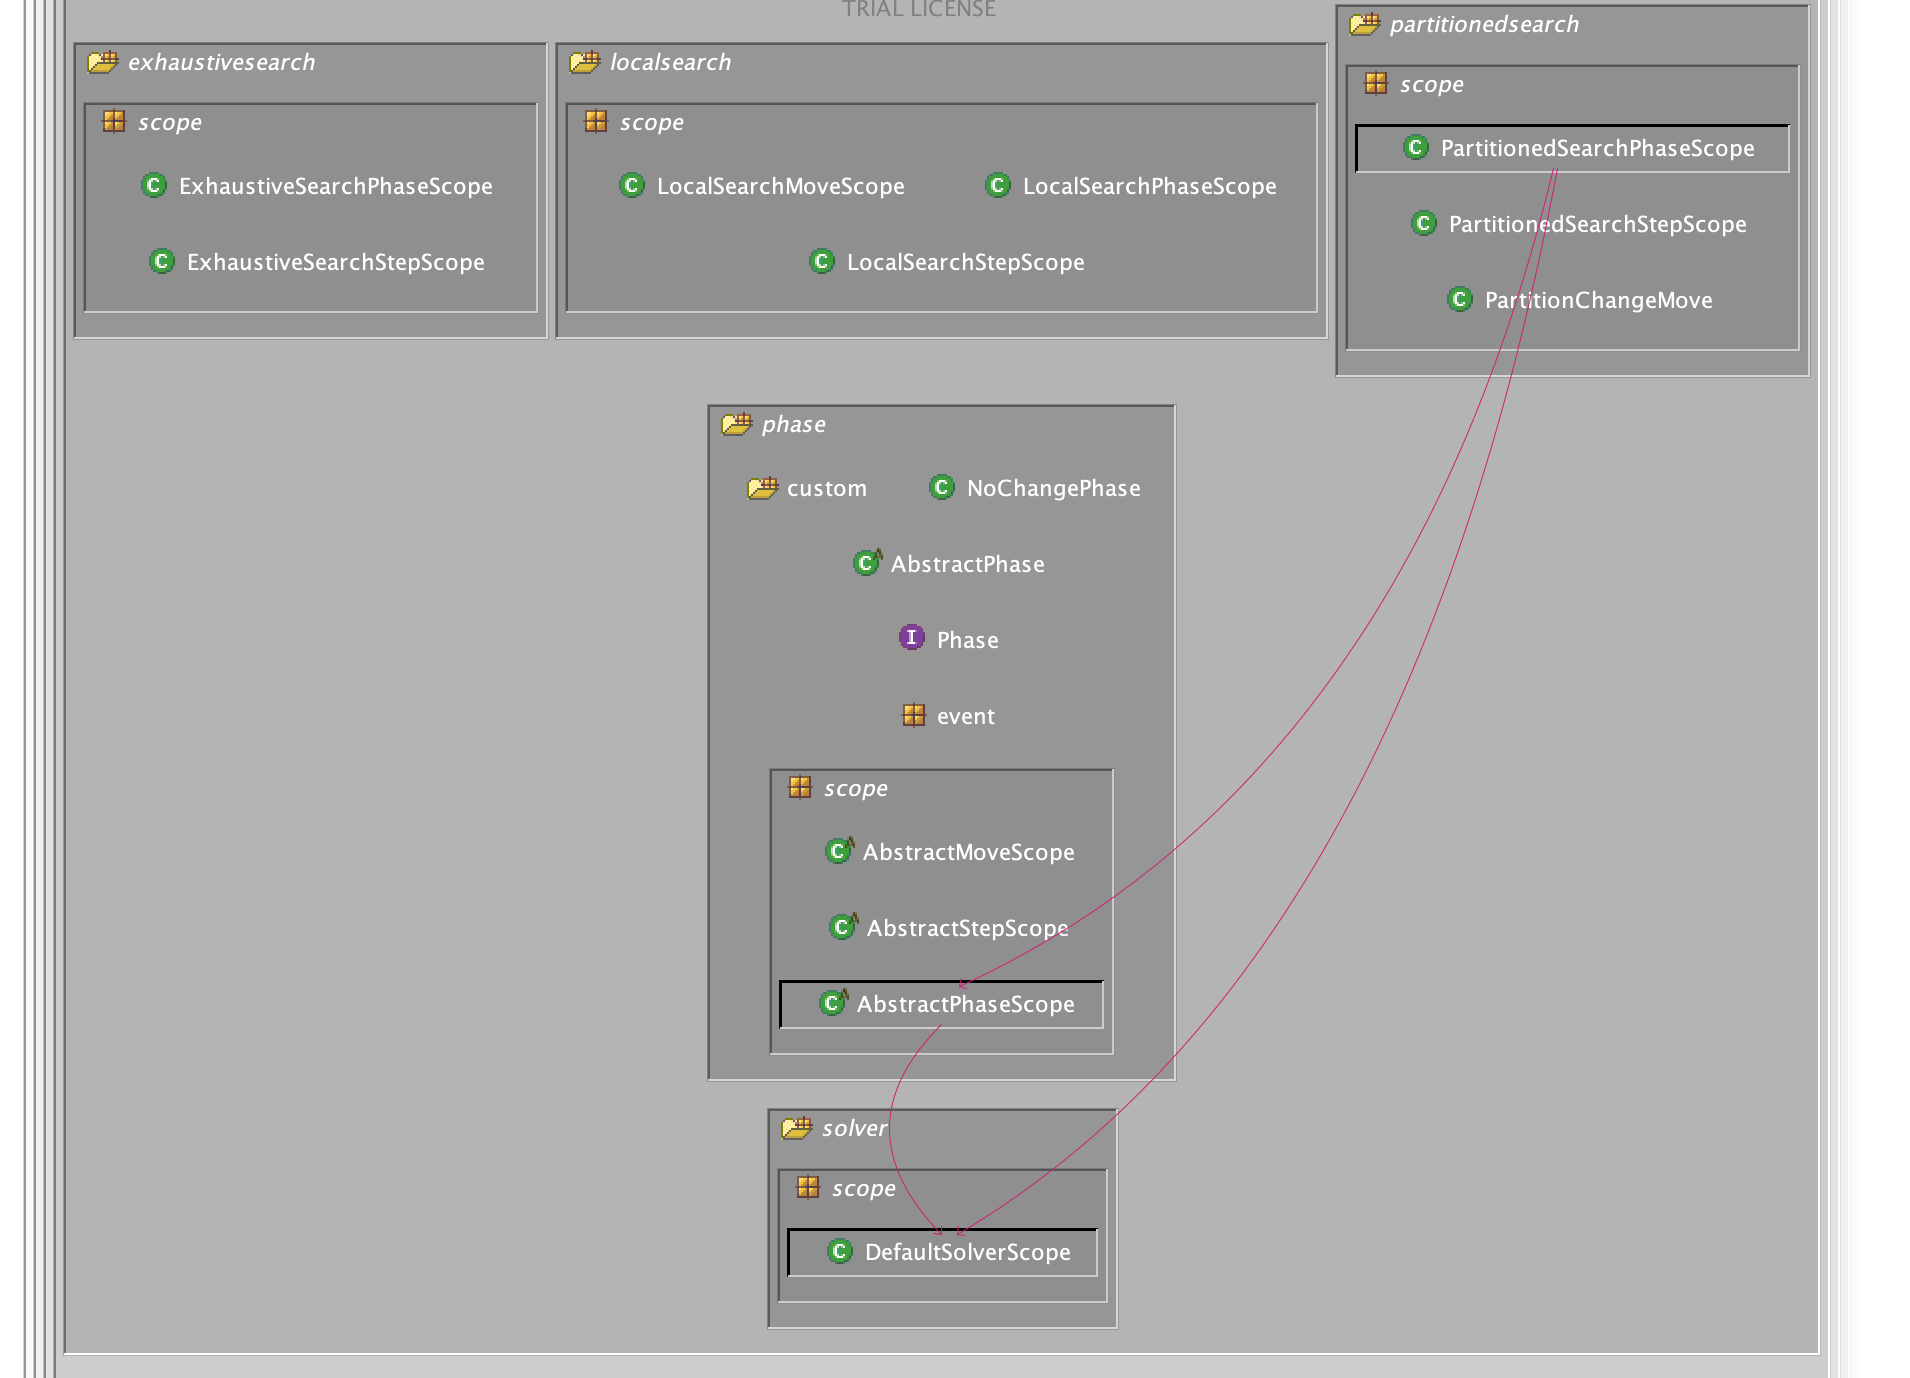
\includegraphics[width=0.8\textwidth]{figures/step2/scope_dep.png}
    \caption{This is a filtered out view of the Implementation system where the focus is placed on the \textit{scope} component of its main entities. Note how the dependencies lay out among the entities. Each entity is dependent on the \textit{solver} scope, while each one of the entities for the \textit{optimization algorithms} are also dependent on the \textit{phase}. We have excluded the dependency flows of the first two algorithms so as not to clutter the figure.}
   \label{fig:impl_scope}
\end{figure}
% C O N F I G
\begin{figure}
    \centering
    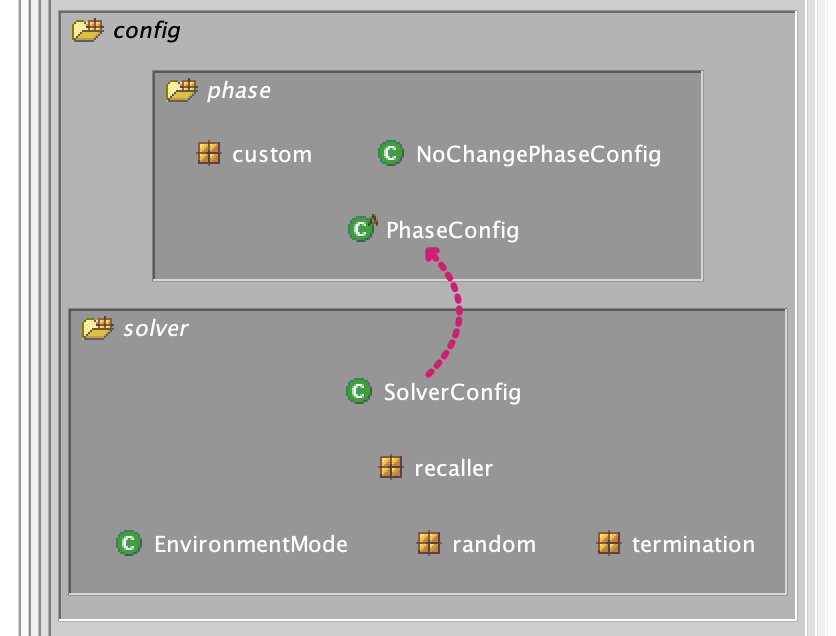
\includegraphics[width=0.6\textwidth]{figures/step2/dep_config.png}
    \caption{This is a close up view on the two main entities of the Configuration system. The arrow depicts dependency. In this case, \textit{SolverConfig} is dependent on \textit{PhaseConfig} because the flow of the arrow is upwards.}
    \label{fig:depend_config}
\end{figure}
% A P I
\begin{figure}
    \centering
    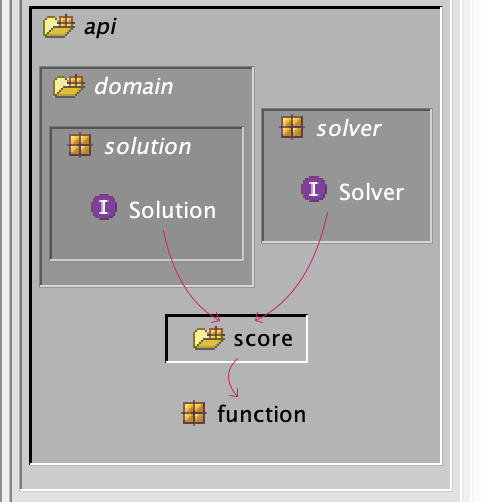
\includegraphics[width=0.5\textwidth]{figures/step2/dep_api.png}
    \caption{This figure depicts the dependency flow between the components of the API. While the \textit{domain} and the \textit{solver} are dependent on the score, the \textit{score} is only dependent on the \textit{function} entity.}
    \label{fig:dep_api}
\end{figure}
%  API AND IMPL
\begin{figure}
    \subfloat[\label{subfig:api-impl-score}This figure depicts the dependency of the API on the Implementation system with regard to the \textit{score} entity. \textit{AbstractBiJoiner} is an abstract class that depends on the abstract class \textit{AbstractJoiner} because it extends it.]{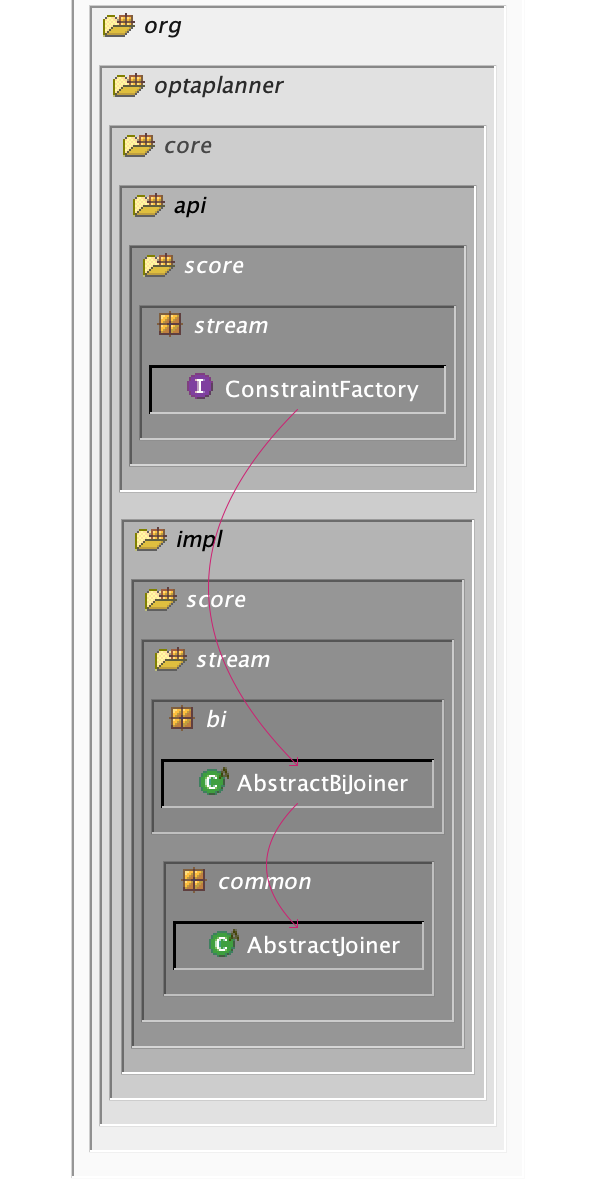
\includegraphics[width=0.4\textwidth]{figures/step2/api_impl_score.png}}
    \hfill
    \subfloat[\label{subfig:api-impl-domain}In this figure we note the dependency of the API based on the domain \textit{entity}.]{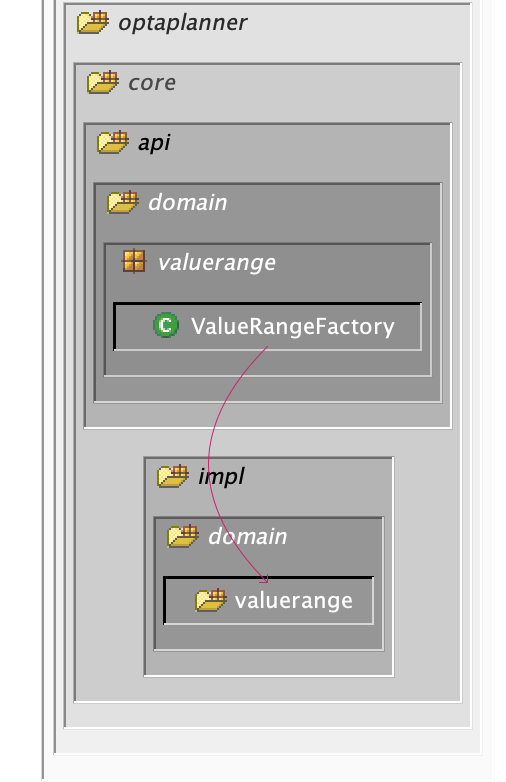
\includegraphics[width=0.48\textwidth]{figures/step2/api_impl_domain.png}}
    \hfill
    \centering
    \subfloat[\label{subfig:impl-api-event}In this figure we note the dependency of the Implementation system on the API based on event listeners. In the current example we note that the main class of an optimization algorithm, \textit{DefaultPartitionedSearchPhase}, uses the event package. This scenario is quite similar for the other two optimization algorithms as well. ]{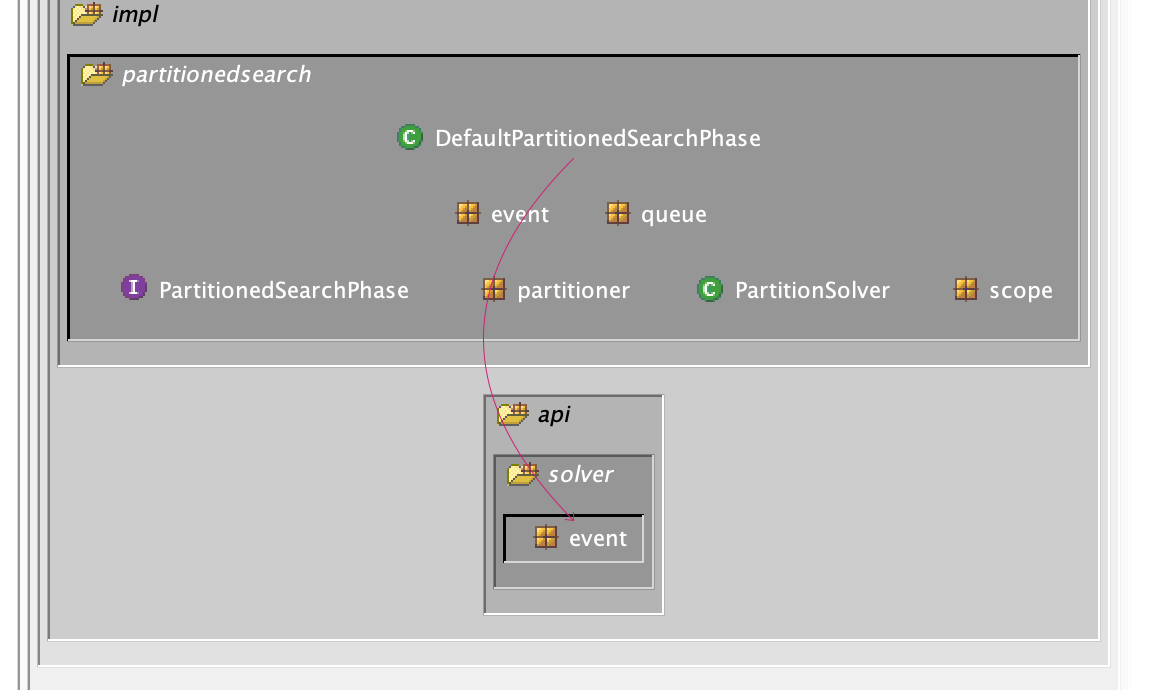
\includegraphics[width=0.6\textwidth]{figures/step2/impl-api-event.png}}
\end{figure}
